\documentclass[doc]{apa6}
\usepackage{lmodern}
\usepackage{amssymb,amsmath}
\usepackage{ifxetex,ifluatex}
\usepackage{fixltx2e} % provides \textsubscript
\ifnum 0\ifxetex 1\fi\ifluatex 1\fi=0 % if pdftex
  \usepackage[T1]{fontenc}
  \usepackage[utf8]{inputenc}
\else % if luatex or xelatex
  \ifxetex
    \usepackage{mathspec}
  \else
    \usepackage{fontspec}
  \fi
  \defaultfontfeatures{Ligatures=TeX,Scale=MatchLowercase}
\fi
% use upquote if available, for straight quotes in verbatim environments
\IfFileExists{upquote.sty}{\usepackage{upquote}}{}
% use microtype if available
\IfFileExists{microtype.sty}{%
\usepackage{microtype}
\UseMicrotypeSet[protrusion]{basicmath} % disable protrusion for tt fonts
}{}
\usepackage{hyperref}
\hypersetup{unicode=true,
            pdftitle={Agreement Attraction},
            pdfauthor={Utku Türk~\& Pavel Logacev},
            pdfborder={0 0 0},
            breaklinks=true}
\urlstyle{same}  % don't use monospace font for urls
\usepackage{biblatex}
\ExecuteBibliographyOptions{maxbibnames=999}
\addbibresource{myreferences.bib}
\addbibresource{r-references.bib}
\usepackage{graphicx,grffile}
\makeatletter
\def\maxwidth{\ifdim\Gin@nat@width>\linewidth\linewidth\else\Gin@nat@width\fi}
\def\maxheight{\ifdim\Gin@nat@height>\textheight\textheight\else\Gin@nat@height\fi}
\makeatother
% Scale images if necessary, so that they will not overflow the page
% margins by default, and it is still possible to overwrite the defaults
% using explicit options in \includegraphics[width, height, ...]{}
\setkeys{Gin}{width=\maxwidth,height=\maxheight,keepaspectratio}
\IfFileExists{parskip.sty}{%
\usepackage{parskip}
}{% else
\setlength{\parindent}{0pt}
\setlength{\parskip}{6pt plus 2pt minus 1pt}
}
\setlength{\emergencystretch}{3em}  % prevent overfull lines
\providecommand{\tightlist}{%
  \setlength{\itemsep}{0pt}\setlength{\parskip}{0pt}}
\setcounter{secnumdepth}{5}
% Redefines (sub)paragraphs to behave more like sections
\ifx\paragraph\undefined\else
\let\oldparagraph\paragraph
\renewcommand{\paragraph}[1]{\oldparagraph{#1}\mbox{}}
\fi
\ifx\subparagraph\undefined\else
\let\oldsubparagraph\subparagraph
\renewcommand{\subparagraph}[1]{\oldsubparagraph{#1}\mbox{}}
\fi

%%% Use protect on footnotes to avoid problems with footnotes in titles
\let\rmarkdownfootnote\footnote%
\def\footnote{\protect\rmarkdownfootnote}


  \title{Agreement Attraction}
    \author{Utku Türk\textsuperscript{1}~\& Pavel Logacev\textsuperscript{1}}
    \date{}
  
\shorttitle{Agreement Attraction in Turkish}
\affiliation{
\vspace{0.5cm}
\textsuperscript{1} Boğaziçi University}
\usepackage{csquotes}
\usepackage{upgreek}
\captionsetup{font=singlespacing,justification=justified}

\usepackage{longtable}
\usepackage{lscape}
\usepackage{multirow}
\usepackage{tabularx}
\usepackage[flushleft]{threeparttable}
\usepackage{threeparttablex}

\newenvironment{lltable}{\begin{landscape}\begin{center}\begin{ThreePartTable}}{\end{ThreePartTable}\end{center}\end{landscape}}

\makeatletter
\newcommand\LastLTentrywidth{1em}
\newlength\longtablewidth
\setlength{\longtablewidth}{1in}
\newcommand{\getlongtablewidth}{\begingroup \ifcsname LT@\roman{LT@tables}\endcsname \global\longtablewidth=0pt \renewcommand{\LT@entry}[2]{\global\advance\longtablewidth by ##2\relax\gdef\LastLTentrywidth{##2}}\@nameuse{LT@\roman{LT@tables}} \fi \endgroup}
\usepackage[utf8]{inputenc}
\usepackage[T1]{fontenc}
\usepackage{xcolor}
\usepackage{hhline}
\usepackage{mathtools}
\linespread{1}
\usepackage{gb4e}
\noautomath
\usepackage{setspace}
\makeatletter
\apptocmd{\@exe}{\singlespacing}{}{}
\makeatother
\usepackage{sectsty}
\allsectionsfont{\large}
\usepackage{color}
\usepackage{hyperref}
\hypersetup{colorlinks = true, linkcolor = blue, citecolor = blue, urlcolor = blue}
\usepackage[english]{babel}
\addto\extrasenglish{\renewcommand{\itemautorefname}{Item}}
\renewcommand*{\nameyeardelim}{\addcomma\space}
\usepackage{tikz}
\usepackage{tikz-qtree}
\let\eachwordone=\textit

\authornote{

Correspondence concerning this article should be addressed to Utku Türk, . E-mail: \href{mailto:utku.turk@boun.edu.tr}{\nolinkurl{utku.turk@boun.edu.tr}}}

\abstract{
The comprehension of agreement within the elements of a sentence is known to fail. One of these comprehension errors is known as agreement attraction. Speakers may erroneously find a sentence in which the ``attractor'' agrees with the verb instead of the ``head'' of the subject. Data from typologically different languages and explanations from different frameworks shows that we are far from understanding by what the attraction is modulated. Some theories refer this phenomenon as a faulty representation of the number on the head of the subject phase whereas other theories argues that the attraction is due to an error in the access to the number of the subject. In this paper, we report two experiments exploring a possible explanation for agreement attraction: an extremely shallow processing. The first experiment is a replication of \textcite{Lago2018} where we changed the head of the subject in order to differentiate between the accusative case \emph{-I}. In the second experiment, we have used a relative clause which only consists of a plural marked verb as a distractor. Our results show that while people do indeed care more than just ``matching'' the forms of plural verbal. Either comprehenders have some sort of restriction to not use cues from verbs upon accessing the number of the plural morpheme or there is a syntactic reason for the number feature of plural morpheme to not ``percolate.''


}

\begin{document}
\maketitle

\hypertarget{introduction}{%
\section{Introduction}\label{introduction}}

\hypertarget{literature}{%
\section{Literature}\label{literature}}

\hypertarget{theories-of-attraction}{%
\subsection{Theories of attraction}\label{theories-of-attraction}}

Agreement attractions are defined as instances of incorrect agreements of an element with a distractor that is not its grammatical controller. As in \autoref{E1}, the target of the agreement is the verb \emph{are}, the attracting distractor is \emph{bottles}, and the feature erroneously assesed is the number feature of the grammatical controller \emph{label}.

\begin{exe}
\ex[*]{The label on the bottles \textit{are} wrong.\footnotemark}
\label{E1}
\end{exe}

\footnotetext{The convention of using $\ast$ is to show the ungrammaticality of the sentencee.}

This type of attraction, called number attraction in subject-verb agreement, first theorized by \textcite{Quirk1972} and attested experimentally by \textcite{Bock1991} in language production. One of the theoretical attempts to explain such phenomenon was Marking and Morphing Theories \autocites{Bock2001}[ among others]{Eberhard2005}. The reason it is called \emph{Marking} and \emph{Morphing} is because there is two possible explanation within the framework with regards to where and when the attraction occurs. First possibility is speaker (and/or comprehender) can erroneously create a semantic representation of the head with wrong number feature in the marking process in the marking process. Another possibility is that the attraction may arise from an interfering number feature of the attractor with the number feature of the highest noun phrase node in morphing process. During the this process, the speaker forms a final number value of the subject phrase, which is determined by each morpheme within the same phrase and their number information with particular weight. In morphing process, these other morphemes with number information may contaminate the final number value with perculation mechanism, which depends on the depth of the syntactic embedding. As the prediction goes, the more embedded an attractor is, the less attraction they trigger as shown in \textcite{Bock1992} in which authors shown that attractors within a relative clause trigger less agreement attraction in the production.

However, other studies shown that other preverbal elements, such as objects, object relative clauses, object clefts, and object questions, may trigger agreement attraction \autocites{Kimball1971}{Hartsuiker2001}{Franck2006}[ among others]{Franck2015}. In sentences like \autoref{E2}, the pronominal object \emph{hen} triggers and agreement attraction without being a part of the subject.

\begin{exe}
\ex[*]{
\gll Theo denkt dat de knecht hen roep.\\
Theo thinks that the servant them call.\textsc{Pl}.\\
\trans  `Theo thinks that the servant \textit{call} them'}
\label{E2}
\end{exe}

Since the Marking and Morphing theories put the source of the agreement attraction on the probe, i.e.~subject phrase, they cannot explain agreement attraction effects that are triggered by an distractor outside of the syntactic scope of the subject. Regardless, these effects can be explained in a framework where the source of the agreement attraction can placed on the trigger, i.e.~verb. \textcite{Badecker2007} suggests that a process where the subject is retrieved from the memory plays a role in agreement attraction effects as well \autocite[see as well][]{Wagers2009}. Building on the work in cue-based retrieval mechanism \autocites{Gordon2001}{Lewis2005}[ among others]{Lewis2006}, they argued that when spakers reach the verb, they try to retrieve the subject using certain features (cues) that essentially marks the \emph{subjecthood}. Thus, any element that matches (or partially mathces) with the cues in use may cause agreement attraction regardless of their position or syntactic relation to the subject. Going back to \autoref{E2}, it is expected, then, for an object which shares features like being preverbal, being a noun phrase, ability to bear agreement with a subject to trigger agreement attraction.

Another challenge for the Marking and Morphing model was the grammaticality asymmetry. Due to the spreading activation formula utilized in the Marking and Morphing model \autocite[see][]{Dell1986}, this model overgeneralizes the attraction effects to both ungrammatical and grammatical sentences and predicts both \autoref{E1} and \autoref{E3} to be present empirically, which is not the case \autocite{Wagers2009}.

\begin{exe}
\ex[*]{The labels on the bottle \textit{is} wrong.}
\label{E3}
\end{exe}

On the other hand, cue-based retrieval models successfully predicts the the grammaticality asymmetry as shown by \textcite{Dillon2013} in an ACT-R simulation as well as numerous studies in self-paced reading, eye-tracking, and ERP studies \autocites{Wagers2009}{Tucker2010}{Tanner2014}[ among others]{Lago2015}. This success was due to their replacement of source of the attraction. According to cue-based retrieval models, the probe, verb, presents certain cues to retrieve an NP with matching features in agreement. When features of the grammatical controller of the verb does not \emph{fully} match with the cues, no single NP will be satisfying the \emph{agreement}. Thus, another NP in the clause can match with cues presented by the VP, such as its case, syntactic position, grammatical number. Thus, if there is no \emph{retrieval cue} in the first place, i.e.~the verb is nor marked plural, there will be no need for partial match.

\hypertarget{turkish-relative-clauses-and-plural-marking}{%
\subsection{Turkish relative clauses and plural marking}\label{turkish-relative-clauses-and-plural-marking}}

Before discussing the experiments, we will touch upon the mechanisms that we utilize in the experiments: optional plural agreement, relative clause structure, and syncretism between possessive and accusative.

Turkish plural agreement is quite similar with regards to the subject-verb number agreement in the first and second plural person. However, Turkish plural agreement is optional in third person plurals as shown in \autoref{TB1} and \autoref{TB2}. The other characteristics of Turkish plural agreement is that, the nominal and verbal plural marking is done by the same morpheme \emph{-lAr}\footnote{The convention of using an uppercase A is to show that the morpheme can surface as either \textit{-ler} or \textit{-lar} according to the previous vowel due to the vowel harmony reasons.}.

\begin{exe}
\ex \label{TB1} Dün çocuk-\textsc{Lar} okul-a git-ti-\textsc{Ler} mi?
\ex 
\gll Dün çocuk-LAR okul-a git-ti mi?\\
yesterday child-\textsc{Pl} school-\textsc{Dat} go-\textsc{Pst}(-\textsc{Pl}) Q\\
\trans ``Did the children go to school yesterday?''
\label{TB2}
\end{exe}

As for Turkish relative clauses, they always precede the external head noun \autocites{Goksel2004}{Taylan2015} and they use either \emph{-An} or \emph{-dIk} nomilizers to show the referentiality of the subject within the relative clause as shown in \autoref{TB3} and \autoref{TB4} \autocite{Haig1997}. Moreover, due to pro-drop and null object properties of the Turkish \autocite[see][]{Ozturk2005}, relative clauses can consist of only the verb itself in Turkish as in \autoref{TB5}.

\begin{exe}
\ex \label{TB3}
\gll Kazı-lar-ın yap-ıl-dığ-ı alan ... \\
excavation-\textsc{Pl}-\textsc{Gen} do-\textsc{Pass}-\textsc{Nmlz}-\textsc{Poss} area ... \\
\glt ``The place where the excavations are done ...''
\ex \label{TB4}
\gll Kazı-lar yap-ıl-an alan ... \\
excavation-\textsc{Pl} do-\textsc{Pass}-\textsc{Nmlz} area ... \\
\glt ``A place where some excavations are done ...''
\ex \label{TB5}
\gll Gör-düğ-ü kuş çok güzel-di.\\
see-\textsc{Nmlz}-\textsc{Poss} bird very pretty-\textsc{Pst}\\
\glt ``The bird that he/she saw was very pretty.''
\end{exe}

Final characteristics that interests us in this paper is the morphological syncretism between the accusative case and possessive suffix in Turkish. When the possessive case is attached to a nominal stem that ends with a consonant, it is pronounced as \textit{-I}, which is exactly how accusative case is also pronounced in the same environment in Turkish. However, the ambiguity is immediately resolved when they follow a nominal stem that ends with a vowel. In the latter environment, the accussative case surfaces as \emph{-yI} whereas the possessive surfaces as \emph{-sI(n)}\footnote{The final \textit{n} is only surfaces when any other morphemes follows the possessive suffix. Otherwise, it surfaces as \textit{-sI}} as shown in \autoref{TB6}-\autoref{TB9}.

\begin{exe}
\ex
\begin{xlist}
\ex \label{TB6}
\gll Kuş-\textbf{u} beğen-di-m.\\
bird-\textsc{Acc} like-\textsc{Pst}-\textsc{1Sg}\\
\glt ``I liked the bird.''
\ex \label{TB7}
\gll Emin'in kuş-\textbf{u} güzel-miş.\\
Emin-\textsc{Gen} bird-\textsc{Poss} pretty-\textsc{Evd}\\
\glt ``Emin's bird was pretty.''
\ex \label{TB8}
\gll Kedi-\textbf{yi} beğen-di-m.\\
cat-\textsc{Acc} like-\textsc{Pst}-\textsc{1Sg}\\
\glt ``I liked the cat.''
\ex \label{TB9}
\gll Emin'in kedi-\textbf{si} güzel-miş.\\
Emin-\textsc{Gen} cat-\textsc{Poss} pretty-\textsc{Evd}\\
\glt ``Emin's cat was pretty.''
\end{xlist}
\end{exe}

\hypertarget{the-current-study}{%
\section{The Current Study}\label{the-current-study}}

In this study, we examine the question of whether agreement attraction is due to the shallow parsing that mainly depends on the memory of plural morpheme \emph{-lAr} and matching the verbal plural morpheme with the nominal plural morpheme.

First of all, we investigate the effects of ambiguous suffix with Experiment 1, which is a replication of \textcite{Lago2018}. \textcite{Lago2018} makes use of genitive-possessive structures in the subject position, in which the possessive-marked noun is the head of the noun phrase which acts as the grammatical agreement controller, and the genitive noun serves as a potential attractor as in \autoref{Lagoitem}. In a speeded acceptability judgment study, \textcite{Lago2018} found a significant effect of number agreement attraction. However, the interpretation of their findings may be a result of the fact that non-subjecthood cues originate from their use of morphologically ambiguous forms of the possessive. In the possessive forms that are used, all the head nouns in their stimuli are ambigiuous between possessive and accusative.

\begin{exe}
\ex \label{Lagoitem}
\gll \c{S}ark{\i}c{\i}-n{\i}n vokalist-i sahne-de s\"{u}rekli z{\i}pla-d{\i}-lar.\\
singer-\textsc{Gen} vocalist-\textsc{Poss} stage-\textsc{Loc} non-stop jump-\textsc{Pst}-\textsc{3Pl}\\
\glt The singer's backup vocalist jumped on the stage non-stop.
\end{exe}

In Turkish, accusative number agreement controllers are extremely rare, while genitive agreement controllers are very frequent. Thus, \textcite{Lago2018}'s finding could potentially be explained with occasional shallow processing. When all syntactic relations in the sentence were processed fully, the possessive noun may have been identified as the controller. Meanwhile, the genitive noun may sometimes have been erroneously identified as the controller during shallow processing because genitives are more likely to act as agreement controllers than accusatives. In order to check this effect, we have replicated \textcite{Lago2018} in Experiment 1. We have used different head nouns which ends with a vowel to differentiate between the accusative case and the possessive suffix, i.e. \emph{taksici} (taxi driver) instead of \emph{vokalist} in \autoref{Lagoitem}.

With regards to percolation theories, this replication should yield no difference from \textcite{Lago2018}. The syntactic depth has not changed, the number information of the head and distractor have not changed. Slight differences may be expected since we have changed some items which can be found in Appendix 1, and this situation can create a erroneous number information to be used in the marking process.

As for cue-based retrieval models, we should expect a lower agreement attraction effect in this replication. This predictions stems from the fact that possibility of erroneous representation of features of head noun is now lower due to our efforts to differentiate between the accusative case and the possessive marking. \textcite{Lago2018} argues that due to the subjecthood information provided by genitive case, there is an effect of agreement attraction. We eliminate the possibility of possible non-subjecthood clues given by the form that is shared by the accusative case and the posessive suffix.

Within the shallow processing model, we would also expect a no change in the status of agreement attraction. In our account of shallow processing, we argue that when the comprehenders reach the verb and saw plural morpheme, they engage in matching mechanism where they try to match the verbal plural morpheme with a previous nomimal plural morpheme. An agreement attraction, then, is not a result of a partial matching or a representational error of number feature; instead, it is the result of a state of memory in which comprehenders misremember either the existence of the nominal plural morpheme or the place of the nominal plural morpheme as stated in the MPT model of the agreement attraction within shallow processor within \autoref{model1}, \autoref{model2}, \autoref{model3}\footnote{Author here wishes he knew more latex to do the MPT tree more neat.}.

\begin{figure}[htb!]
\centering
\begin{tikzpicture}[
    sibling distance        = 0.5em,
    level distance          = 5em,
    edge from parent/.style = {draw, -latex},
    every node/.style       = {font=\scriptsize},
    sloped
  ]
\Tree [.{\ }
        \edge node[auto=left]{f}; [.\node[draw,rounded corners=.8ex]{generic failure};
                                     \node[draw]{Ungrammatical};]
        \edge node[auto=left]{1-f};
        [.\node[draw,rounded corners=.8ex]{no failure};
          \edge[dashed]; [.\node[]{Plural Verbs}; 
                           \edge[dashed]; \node[]{With Distractor};
                           \edge[dashed]; \node[]{Without Distractor};
                         ] 
          \edge[dashed]; [.\node[]{Singular Verbs}; 
                          \edge[dashed]; [.\node[draw,rounded corners=.8ex]{No checking};
                                           \node[draw]{Grammatical};]
                         ] 
        ] 
      ]
\end{tikzpicture}
\caption{xd}
\label{model1}
\end{figure}

\begin{figure}[htb!]
\centering
\begin{tikzpicture}[
    sibling distance        = 0.5em,
    level distance          = 5em,
    edge from parent/.style = {draw, -latex},
    every node/.style       = {font=\scriptsize},
    sloped
  ]
\Tree [.\node[]{Without Distractor}; 
                                          \edge node[auto=left]{m$_2$}; [.\node[draw,rounded corners=.8ex]{No Memory of -lAr};
                                                                        \edge node[auto=left]{g}; \node[draw]{Grammatical};
                                                                        \edge node[auto=left]{1-g}; \node[draw]{Ungrammatical};]
                                          \edge node[auto=left]{1-m$_2$}; [.\node[draw,rounded corners=.8ex]{Memory of -lAr}; 
                                          \edge node[auto=left]{1-p$_2$}; [.\node[draw,rounded corners=.8ex]{No Place of -lAr};
                                                                        \edge node[auto=left]{g}; \node[draw]{Grammatical};
                                                                        \edge node[auto=left]{1-g}; \node[draw]{Ungrammatical};]
                                          \edge node[auto=left]{p$_2$}; [.\node[draw,rounded corners=.8ex]{Misrepresented place of -lAr};
                                                                        \node[draw]{Ungrammatical};]]]
                                                                        
                                                                    
                                                                    
\end{tikzpicture}
\caption{xd}
\label{model2}
\end{figure}
\begin{figure}[htb!]
\centering
\begin{tikzpicture}[
    sibling distance        = 0.5em,
    level distance          = 5em,
    edge from parent/.style = {draw, -latex},
    every node/.style       = {font=\scriptsize},
    sloped
  ]
\Tree [.\node[]{With Distractor}; 
                                          \edge node[auto=left]{m$_1$}; [.\node[draw,rounded corners=.8ex]{No Memory of -lAr};
                                                                        \edge node[auto=left]{g}; \node[draw]{Grammatical};
                                                                        \edge node[auto=left]{1-g}; \node[draw]{Ungrammatical};]
                                          \edge node[auto=left]{1-m$_1$}; [.\node[draw,rounded corners=.8ex]{Memory of -lAr}; 
                                          \edge node[auto=left]{1-p$_1$}; [.\node[draw,rounded corners=.8ex]{No Place of -lAr};
                                                                        \edge node[auto=left]{g}; \node[draw]{Grammatical};
                                                                        \edge node[auto=left]{1-g}; \node[draw]{Ungrammatical};]
                                          \edge node[auto=left]{p$_1$}; [.\node[draw,rounded corners=.8ex]{Memory of place of -lAr};
                                                                        \node[draw]{Grammatical};]]]
                                                   
\end{tikzpicture}
\caption{xd}
\label{model3}
\end{figure}

In our second experiment, we investigate the predictions made from our model using a verbal plural morpheme within a distractor relative clause. As mentioned earlier, the verbal plural morpheme in Turkish is exactly the same with the nominal plural with regards to its stress, its behaviour, and its form: \emph{-lAr}. Since Turkish relative clauses are essentially nominals due the nomilization process, they behave exactly like other nominals within the sentence \autocites{Goksel2004}{Taylan2015}. They can be marked with cases, plural agreement and they can have postpositions that any nominal also can. This syntactic formation enables us to question how shallow people process, how much syntactic information is relevant, or how perfectly people encode the features of the elements of the sentence. In our experiment 2, we have used items in which the referential head noun of the subject is modified with a single-word relative clause as in \autoref{ouritem1}.

\begin{exe}
  \ex \label{ouritem1}
      \gll D\"{o}v-d\"{u}k-(\textbf{ler})-i \c{c}ocuk mutfak-ta bayg{\i}n hal-de yat-{\i}yor-(\textbf{lar})-d{\i}.\\
  beat-\textsc{Nmlz}-(\textsc{Pl})-\textsc{Poss} kid kitchen-\textsc{Loc} unconscious state-\textsc{Loc} lie-\textsc{Prog}-(\textsc{Pl})-\textsc{Pst}\\
      \glt Intended: The kid that they beat were laying in the kitchen unconscious.
\end{exe}

Within the framework of percolation theories, we expect a harsh decline in the agreement attraction effects\footnote{Discussion regarding to the how and where relative clauses adjoined is omited due to the scope of the paper. However, it should be clear that a late insertion analysis where the relative clauses are actually above the head noun would yield different results. In this paper, I assume that modifiers like relative clauses are within the noun phrase, which deems them \textit{syntactically} deeper placed in the hierarchical three than the possessee.}. The reason for this expected decline is the fact that relative clauses being relative \emph{deeper} in the hierarchical structure than the possessee of genitive-posessive structure.

As for cue-based retrieval models, we would expect an agreement attraction quite similar to the one that we originally have in \textcite{Lago2018}. The reason for this expected agreement attraction is the fact that apart from having a verbal root, the relative clauses and nomials are behave exactly the same in terms of \emph{nounnness}. Like nominals, nominalized structures first marked with plural and then with the case or possessive suffix. From this aspective, it seems like there should be no difference. However, one may argue that the features related to the verbal and nominal can be encoded differently. Thus, there will no partial match at any time given due to the fact that verbal plural morpheme at the main verb does specify cues for specific type of plural marking. One other question that may arise from this structure is that whether or not the parts of already-formed dependencies can feed the following dependency resolution. In other words, the verbal plural morpheme \emph{-lar} on \emph{dövdükleri} in \autoref{ouritem1} is already a trigger of a cue retrieval process. And, when it is merged with the nominal head \emph{çocuk}, there is a formed semantic meaning that is \enquote{a group of people have beaten a kid.} However, this \emph{suggesstion} assumes that relative clauses are formed at the very moment. Moreover, we also need to assume that after forming a relative clause they are unreachable, meaning that they do not contribute to the processing of the sentnece, anymore.

Lastly in our extremely shallow processing model, we would expect a significant effect of agreement attraction. Due to one of the writers inability to \emph{run the numbers} and \emph{form the mpt trees in time}, this part unfortunately does not go beyond than a verbal argumentation. The reason we wait a significant effect of agreement is due to the fact that upon the agreement process is driven by the faulty memory of the place of the plural morpheme and uneducated guessing. Since the parsing is shallow, comprehenders do not engage in perfect attribution of the features, thus having a somewhat blurry representation behind. We expect for this behaviour to be omnipresent in other agreement attraction phenomenon that has been showed, as well as in \textcite{Lago2018} and in our replication of it. Therefore, there is no reason to have to anything to be different in experiment 2.

\hypertarget{experiment-1}{%
\subsection{Experiment 1}\label{experiment-1}}

In their study, \textcite{Lago2018} investigates the comprehension of subject-verb agreement Turkish monolinguals. They use speeded acceptability judgments for the effects of number attraction in Turkish. Their sentences make us of genitive-possessive constructions in the subject position, where the genitive is the attractor and the possessive is the head noun. They manipulate the grammaticality of the sentence by changing the plural morphology of the verb, and they also manipulate the plurality of the attractor noun. In grammatical conditions, the subject and the verb both bear singular morphology with no overt morpheme. Moreover, in the ungrammatical conditions, the verb bears the overt \emph{-lAr} morpheme whereas the subject is still singular as exemplified below.

\begin{exe}
\ex
\begin{xlist}

\ex \textsc{Ungrammatical, SG attractor} \label{lago4}
\gll \c{S}ark{\i}c{\i}-n{\i}n vokalist-i sahne-de s\"{u}rekli z{\i}pla-d{\i}-lar.\\
singer-\textsc{gen} vocalist-\textsc{poss} stage-\textsc{loc} non-stop jump-\textsc{pst}-\textsc{3Pl}\\
\glt The singer's backup vocalist jumped on the stage non-stop.

\ex \textsc{Grammatical, PL attractor} \label{lago2}
\gll \c{S}ark{\i}c{\i}-lar-{\i}n vokalist-i sahne-de s\"{u}rekli z{\i}pla-d{\i}\\
singer-\textsc{pl}-\textsc{gen} vocalist-\textsc{poss} stage-\textsc{loc} non-stop jump-\textsc{pst}-$\varnothing$\\
\glt The singers' backup vocalist jumped on the stage non-stop.


\ex \textsc{Ungrammatical, PL attractor} \label{lago3}
\gll \c{S}ark{\i}c{\i}-lar-{\i}n vokalist-i sahne-de s\"{u}rekli z{\i}pla-d{\i}-lar.\\
singer-\textsc{pl}-\textsc{gen} vocalist-\textsc{poss} stage-\textsc{loc} non-stop jump-\textsc{pst}-\textsc{3Pl}\\
\glt The singers' backup vocalist jumped on the stage non-stop.

\ex \textsc{Grammatical, SG attractor} \label{lago1}
\gll \c{S}ark{\i}c{\i}-n{\i}n vokalist-i sahne-de s\"{u}rekli z{\i}pla-d{\i}\\
singer-\textsc{gen} vocalist-\textsc{poss} stage-\textsc{loc} non-stop jump-\textsc{pst}-$\varnothing$\\
\glt The singer's backup vocalist jumped on the stage non-stop.

\end{xlist}
\end{exe}

They found a significant effect of number attraction in Turkish ranging between 11\%--15\% across monolinguals. \textcite{Lago2018} stipulate that the Turkish genitive case does not provide a strong cue against subjecthood since Turkish frequently makes use of genitive marked subjects in embedded clauses, as in \autoref{gensubj}. This is in contrast with English, in which the genitive case is compatible with subjecthood. Thus, \textcite{Lago2018} argue that this robust agreement attraction effect has been linked to the case information carried by accusative and genitive.

\begin{exe}
\ex \label{gensubj}
\gll k\"{o}y-\"{u} bir haydut-un bas-t{\i}\u{g}-{\i}n-{\i} duy-du-m.\\
village-\textsc{acc} a bandit-\textsc{gen} raid-\textsc{nmlz}-\textsc{3Sg}-\textsc{acc} hear-\textsc{pst}-\textsc{1Sg}\\
\glt I heard that a (certain) robber raided the village. (Adapted from Woolford (2009))
\end{exe}

However, our initial hypothesis postulates that participants engage in shallow processing, which results in a situation in which not only the genitive case but also the possessive case plays a significant role in delivering the case information. None of the experimental items in \textcite{Lago2018} have a head noun which ends with a vowel; thus, all of the possessive markers are morphologically and phonologically ambiguous between the accusative case and the possessive. Unlike genitive case, it is extremely rare for the accusative case to appear on the head noun of the subject, which only occurs in raising predicates as in \autoref{dsm}.

\begin{exe}
\ex \label{dsm}
\gll Ben sen-i git-ti-n san-d{\i}-m\\
I you-\textsc{acc} go-\textsc{pst}-\textsc{2Sg} suppose-\textsc{pst}-\textsc{1Sg}\\
\glt I thought you were gone.
\end{exe}

In order to test this hypothesis, we have replicated the experiment of \textcite{Lago2018} with modified items, in which the possessive is not ambiguous with the accusative case. We tried to be as faithful as possible to the original sentences while also trying to make the sentences as plausable as possible. We keep the semantic relation between the head noun and the controller the same with what has been described in \textcite{Lago2018}, which is either a relation regarding profession or a service that is given by the head noun for the possessor. A set of sentences are exemplified below.

\begin{exe}
\ex
  \begin{xlist}
  \ex \underline{Ungrammatical, PL attractor} \label{exp3}
      \gll Komedyen-ler-in yard{\i}mc{\i}-s{\i} poyraz-dan dolayi \"{u}\c{s}\"{u}-d\"{u}-ler.\\
  comedian-\textsc{pl}-\textsc{gen} helper-\textsc{poss} northeaster-\textsc{abl} because.of feel.chilly-\textsc{pst}--\textsc{pl}\\
      \glt Because of the northeaster, comedians' assistant felt chilly.

  \ex \underline{Grammatical, PL attractor} \label{exp2}
      \gll Komedyen-ler-in yard{\i}mc{\i}-s{\i} poyraz-dan dolayi \"{u}\c{s}\"{u}-d\"{u}.\\
  comedian-\textsc{pl}-\textsc{gen} helper-\textsc{poss} northeaster-\textsc{abl} because.of feel.chilly-\textsc{pst}-$\varnothing$\\
      \glt Because of the northeaster, comedians' assistant felt chilly.

  
  \ex \underline{Ungrammatical, SG attractor} \label{exp4}
      \gll Komedyen-in yard{\i}mc{\i}-s{\i} poyraz-dan dolayi \"{u}\c{s}\"{u}-d\"{u}-ler.\\
  comedian-\textsc{gen} helper-\textsc{poss} northeaster-\textsc{abl} because.of feel.chilly-\textsc{pst}-\textsc{pl}\\
      \glt Because of the northeaster, comedian's assistant felt chilly.
  
  \ex \underline{Grammatical, SG attractor} \label{exp1}
      \gll Komedyen-in yard{\i}mc{\i}-s{\i} poyraz-dan dolayi \"{u}\c{s}\"{u}-d\"{u}.\\
  comedian-\textsc{gen} helper-\textsc{poss} northeaster-\textsc{abl} because.of feel.chilly-\textsc{pst}-$\varnothing$\\
      \glt Because of the northeaster, comedian's assistant felt chilly.

  \end{xlist}
\end{exe}

As seen in the examples, unlike \textcite{Lago2018}'s experimental items, all of our items bear the \emph{-sI} possessive marker instead of the ambiguous \emph{-I} marker. As for the filler items, we could not use or modify the original experiment items since the fillers of the original study were not online. We have used two types filler sentences: grammatical sentences in which the verb bears plural agreement (\autoref{fillera}), and ungrammatical sentences in which the verb does not bear plural agreement (\autoref{fillerb}). We wanted to nullify a possible strategy by the participants where they associate the sentence-final morpheme directly with the acceptability of the sentence. And we also wanted to eliminate the possibility of participants disregarding other elements in the sentences while answering the questions we ask right after the sentence.

\begin{exe}
\ex
\begin{xlist}
\ex \label{fillera}
\gll Adam-{\i}n anne-si fena-la\c{s}-{\i}nca inek kurban et-ti-ler.\\
man-\textsc{gen} mother-\textsc{poss} bad-\textsc{vrb}-\textsc{cvb} cow sacrifice do-\textsc{pst}-\textsc{pl}\\
\glt When his mother got ill, (they) sacrificed a cow.
\ex \label{fillerb}
\gll *Pizzac{\i}-n{\i}n kurye-si t\"{o}kezle-yince sos-lar yer-e sa\c{c}-t{\i}.\\
pizzaria-\textsc{gen} courier-\textsc{poss} trip-\textsc{cvb} sauce-\textsc{pl} floor-\textsc{dat} scatter-\textsc{pst}\\
\glt Intended: When the pizza boy tripped, sauces scattered around. 
\end{xlist}
\end{exe}

\hypertarget{participants-and-procedure}{%
\subsubsection{Participants and Procedure}\label{participants-and-procedure}}

One hundred and seven Turkish speakers were recruited from Bogazici University in İstanbul. We did not collect participants' knowledge of other languages; however, we verified that Turkish is their native language and that they predominantly use it in their daily lives. In the experiments, participants were asked to judge the acceptability of experimental and filler sentences in Turkish. All of the sentences were presented one word at a time in the center of the screen for 500 ms per word unlike \textcite{Lago2018} and \textcite{Wagers2009}, in which the duration was 300 ms per word. The experiment was run on a web-based platform titled the Ibex Farm, and all of the documentation can be found on our github page.

Before the experiment, participants were instructed to give accurate and quick answers based on their own intuitions, and they were also notified about the time limit for answering. At the start of the experiment, they were given 4 practice items with feedback. Each trial after the practice items started with a blank screen, followed by a flash of single words in the middle of the screen. After the sentence, they were asked a grammaticality judgment questins (Was the sentence you read was natural to you?) where they need to press P for \emph{no} and press Q for \emph{yes}. In the experiment, every participant saw 40 experimental item that is latin-squared and 40 fillers.

\hypertarget{analysis}{%
\subsubsection{Analysis}\label{analysis}}

Every experimental item from both experiments (Experiment 1 and \textcite{Lago2018}) is included in the analysis. Participants that could not exceed the threshold of 0.25 difference in \emph{yes} answer between the condition (c) and (d), namely Ungrammatical, SG attractor and Grammatical, SG attractor, were excluded. We performed an analysis by fitting linear mixed-effect modelts to our data, controlling for vowel ending, plural attractor, grammaticality and their interactions. Models were fit using bernoulli distribution with probit link function and 95\% confidence intervals.

\hypertarget{results}{%
\subsubsection{Results}\label{results}}

\begin{figure}
\centering
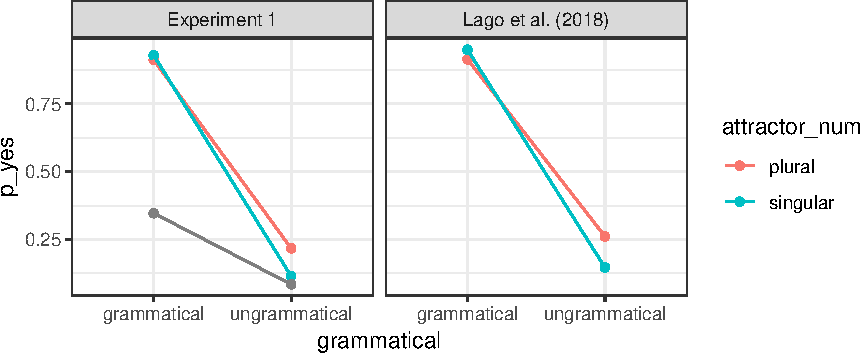
\includegraphics{AgreementAttraction_files/figure-latex/exp1AvgResponse-1.pdf}
\caption{\label{fig:exp1AvgResponse}Estimates and 95\% credible intervals for the analysis of the probability of a \enquote{yes} response.}
\end{figure}

In Figure \ref{fig:exp1AvgResponse}, the y-axis shows the percentage of \enquote{acceptable} answers, and the x-axis indicates whether or not the sentences in that group are grammatical. As seen in the figure, 0.22\% of the sentences with plural attractors and a singular verb were accepted by the participants, in line with the findings of \textcite{Lago2018}. We also see a number attraction rate of 0.11\% which was also observed in \textcite{Lago2018} with close results.

In Figure \ref{fig:exp1ResponseModelPlot}, we clearly see the effects of ungrammaticality and the interaction between the ungrammaticality and plural attractor. We see that, vowel ending is not significant even though it has negative effect. Thus, we may say that differentiating between the accusative case and the possessive suffix has cause a reduction in the effect of the agreement attraction. The results also shows that when the attractor is plural, people have a high tendency to find the sentence grammatical.

\begin{figure}
\centering
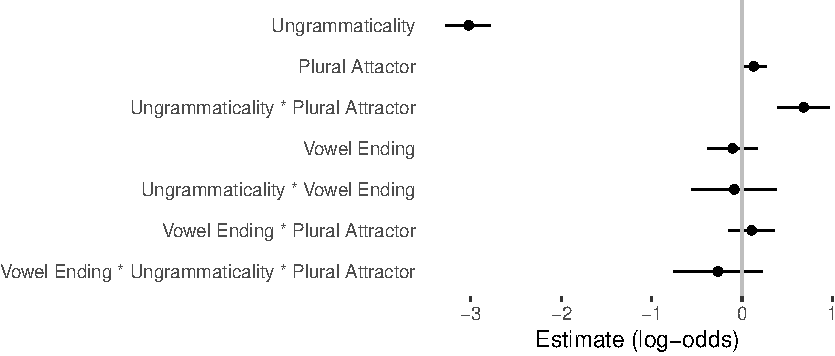
\includegraphics{AgreementAttraction_files/figure-latex/exp1ResponseModelPlot-1.pdf}
\caption{\label{fig:exp1ResponseModelPlot}log-odd Estimates and 95\% credible intervals for the regression coefficients.}
\end{figure}

In Figure \ref{fig:exp1AvgRTs}, we see that average response times are significantly higher than the those of \textcite{Lago2018}. Again, these results shows the effect of disambiguation of the possessive suffix from the accusative case has surfaced as the difficuilty in response and memory retrieval time.

\begin{figure}
\centering
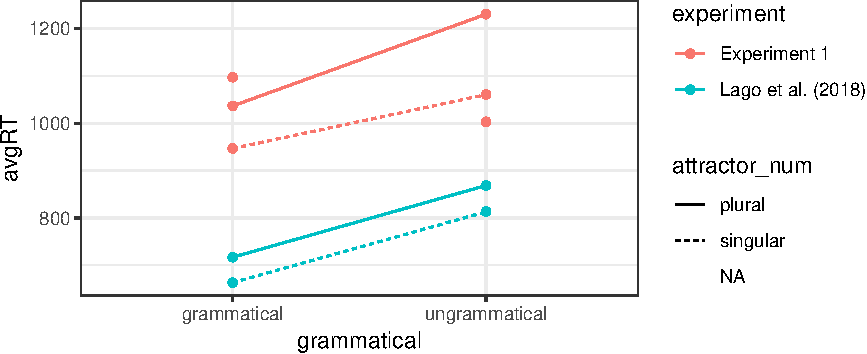
\includegraphics{AgreementAttraction_files/figure-latex/exp1AvgRTs-1.pdf}
\caption{\label{fig:exp1AvgRTs}Average response times for our replication and Lago et. al. (2018)}
\end{figure}

\hypertarget{discussion}{%
\subsubsection{Discussion}\label{discussion}}

The results follow from what a cue-based model would predict: slightly lower agreement attraction. However, these results can also be a result of a badly formed filler sentences which are shown with purple line. Participants may be biased towards saying no since most of the experimental items being ungramatical. However, this can also be statistical \emph{miss} since we may accidentally have a group such as this one. However, the visible effect of vowel ending and response time suggest that people do indeed care more than only the retrieval of plural morpheme \emph{-lar} and its place. This results go against what we have predicted for the Marking and Morphing model and our shallow processing model. However, the existence of extremely close degree of agremeent attraction effects and non-significant nature of the effect of the vowel ending indicate that we cannot readily discard other explanations.

\hypertarget{experiment-2}{%
\subsection{Experiment 2}\label{experiment-2}}

Having discussed the replication study of \textcite{Lago2018}, we have shown that results favor the cue-based models, especially with the effect of disambiguated possessive suffix on response times. However, due to the extremely similar effects on agreement attraction we can still entartain shallow processing mechanism as explained in \autoref{model1}, \autoref{model2}, and \autoref{model3}. Since we argue that the agreement attraction is a product of memory state in which comprehenders do not have an exact memory of the place of the plural morpheme mainly, we conducted an experiment where the distractor with the plural morpheme in on the relative clause.

The study consists of an speeded acceptability judgment experiment in the web-based platform Ibex Farm. In the experiment, we test whether or not speakers utilize even more shallow parser than what is stipulated by \textcite{Lago2018} and our replication of \textcite{Lago2018} Experiment 2. This was investigated using syntactic structures similar to \textcite{Lago2018} materials, in which we have opted out the Genitive Constructuion (GC) for Relative Clause construction (RCC) as a distractor. In Turkish, like GC, relative clause in RCC precedes the head noun, and length-wise Turkish relative clauses can consist of only one word and the rest can be dropped. Turkish allows us to use RCCs as distractors in the same place because Turkish plural morpheme in verbal domain and nominal domain are the same: \emph{-lAr}. Both of them react similarly in the same phonological environments, and they also exhibit same stress patterns.

In the experimental items, the distractor RC and the matrix verb had four configurations in which the number morpheme on the RCC (\emph{plural} vs. \emph{singular} marked RC verb) and matrix verb (\emph{grammatical} vs. \emph{ungrammatical}) as in \autoref{prereg1}.

\begin{exe}
\ex \label{prereg1}
  \begin{xlist}
  \ex \underline{Grammatical, SG attractor} \label{reg1}
      \gll D\"{o}v-d\"{u}\u{g}-\"{u} \c{c}ocuk okul-a yorgun arg?n gel-di.\\
  beat-\textsc{nmlz}-\textsc{poss} kid school-\textsc{dat} unconscious state-\textsc{loc} lie-\textsc{prog}-\textsc{pst}\\ 
      \glt The kid that he/she beats was laying in the kitchen unconscious.
  \ex \underline{Grammatical, PL attractor} \label{reg2}
      \gll D\"{o}v-d\"{u}k-ler-i \c{c}ocuk mutfak-ta bayg{\i}n hal-de yat-{\i}yor-du.\\
  beat-\textsc{nmlz}-\textsc{pl}-\textsc{poss} kid kitchen-\textsc{loc} unconscious state-\textsc{loc} lie-\textsc{prog}-\textsc{pst}\\
      \glt The kid that they beat was laying in the kitchen unconscious.
  \ex \underline{Ungrammatical, PL attractor} \label{reg3}
      \gll D\"{o}v-d\"{u}k-ler-i \c{c}ocuk mutfak-ta bayg{\i}n hal-de yat-{\i}yor-lar-d{\i}.\\
  beat-\textsc{nmlz}-\textsc{pl}-\textsc{poss} kid kitchen-\textsc{loc} unconscious state-\textsc{loc} lie-\textsc{prog}-\textsc{pl}-\textsc{pst}\\
      \glt Intended: The kid that they beat were laying in the kitchen unconscious.
  \ex \underline{Ungrammatical, SG attractor} \label{reg4}
      \gll D\"{o}v-d\"{u}\u{g}-\"{u} \c{c}ocuk mutfak-ta bayg{\i}n hal-de yat-{\i}yor-lar-d{\i}.\\
  beat-\textsc{nmlz}-\textsc{poss} kid kitchen-\textsc{loc} unconscious state-\textsc{loc} lie-\textsc{prog}-\textsc{pl}-\textsc{pst}\\
      \glt Intended: The kid that he/she beats were laying in the kitchen unconscious.
  \end{xlist}
\end{exe}

As for the experiment, we have used same type of fillers with the Experiment 1 in order to tackle with two possible strategies that can be utilized by the participants: (i) deeming the sentence acceptable when the matrix verb is singular and (ii) deeming most of the sentences unacceptable when the matrix verb is plural. To tackle with the first type of strategy, we have used a sentence where the object is not marked with accusative and it is not in immediately pre-verbal position as in \autoref{filler1a}. The idea was to have a singular matrix verb in an ungrammtical sentence where the ungrammaticality does not stem from the local elements. As for the other strategy we have used pro-drop charactheristics of Turkish and made the first noun phrase with a relative clause an object as in \autoref{filler1b}. The idea behind is that the plural agreement on the matrix verb is resolved with a dropped subject instead of the first noun phrase with a relative clause. Every participant saw 40 experimental item that is latin-squared and 40 fillers.

\begin{exe}
\ex
\begin{xlist}
\ex \label{filler1a}
\gll * Haberleş-tiğ-i çevirmen ara-ma-yınca metin keyfince bitir-di.\\
{\ } communicate-\textsc{Nmlz}-\textsc{Poss} translator call-\textsc{Neg}-\textsc{Nmlz} text as.he.wished finis-\textsc{Pst}\\
\glt Intended: ``When the translator that he spoke with did not call, he finished the text as he wished.''
\ex \label{filler1b}
\gll Sev-dik-ler-i öğretmen emekli ol-unca saatlerce ağla-dı-lar.\\
love-\textsc{Nmlz}-\textsc{Pl}-\textsc{Poss} teacher retired be-\textsc{Nmlz} for.hours cry-\textsc{Pst}-\textsc{Pl}\\
\glt ``When the teacher they loved retired, they cried for hours.''
\end{xlist}
\end{exe}

\hypertarget{participants-and-procedure-1}{%
\subsubsection{Participants and Procedure}\label{participants-and-procedure-1}}

Eighty Turkish speakers were recruited from Bogazici University in İstanbul. The procedure was exatcly the same as the Experiment 1. The participants in this experiment were completely different than the Experiment one.

\hypertarget{analysis-1}{%
\subsubsection{Analysis}\label{analysis-1}}

Every experimental item from both experiments (this experiment and the Experiment 1) is included in the analysis. Participants that could not exceed the threshold of 0.25 difference in \emph{yes} answer between the condition (c) and (d), namely Ungrammatical, SG attractor and Grammatical, SG attractor, were excluded. We performed an analysis by fitting linear mixed-effect modelts to our data, controlling for vowel ending, plural attractor, grammaticality and their interactions. Models were fit using bernoulli ditribution with probit link function and 95\% confidence intervals.

\hypertarget{results-1}{%
\subsubsection{Results}\label{results-1}}

\begin{figure}
\centering
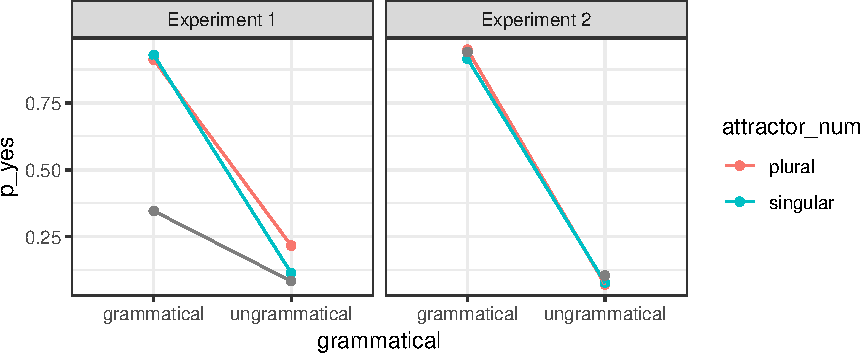
\includegraphics{AgreementAttraction_files/figure-latex/exp2AvgResponse-1.pdf}
\caption{\label{fig:exp2AvgResponse}Estimates and 95\% credible intervals for the analysis of the probability of a \enquote{yes} response.}
\end{figure}

It is clear from Figure \ref{fig:exp2AvgResponse} that in the condition (c) where we expect an agreement attraction, participants find as unacceptable as the condition (d) with singular attractor, singular head noun, and plural matrix verb. While we do not see any agreement attraction (0.07\%), we also see a more firm analysis of the ungrammatical sentence with singular matrix verb ((0.07\%)).

As for the estimates of coefficients in \ref{fig:exp2ResponseModelPlot}, we can conclude that there is a significant negative effect of plural morpheme on the relative clause, which means that it does not cause any agreement affects. Again, the effect of ungrammaticality that stems from the existence of plural morpeheme on the matrix verb is visible. The interaction between the plural morpheme on the attractor RC and the matrix verb is even higher than the sole effect of plural morpheme on the attractor RC.

\begin{figure}
\centering
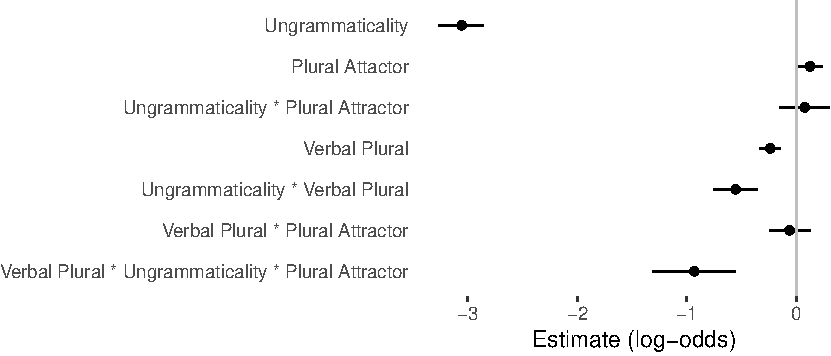
\includegraphics{AgreementAttraction_files/figure-latex/exp2ResponseModelPlot-1.pdf}
\caption{\label{fig:exp2ResponseModelPlot}log-odd Estimates and 95\% credible intervals for the regression coefficients.}
\end{figure}

\begin{figure}
\centering
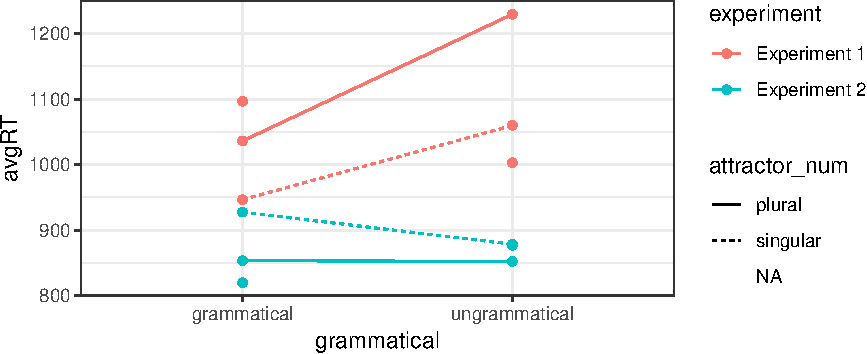
\includegraphics{AgreementAttraction_files/figure-latex/exp2AvgRTs-1.pdf}
\caption{\label{fig:exp2AvgRTs}Average response times for our replication and Experiment2}
\end{figure}

Finally, the response times of the Experiment 2 is significantly lower than the Experiment 1 as seen from Figure \ref{fig:exp2AvgRTs}. The even lower response time in ungrammatical plural (condition c) shows that participants were extremely confident with their decision and did not had any issue with the dependency resolution.

\hypertarget{discussion-1}{%
\subsubsection{Discussion}\label{discussion-1}}

These findings indicate that our hypothesis regarding the matching of the forms is not supported by the empirical evidence. However, results in Experiment 2 points in a direction where the Marking and Morphing studies predicted in the first place. Due to the deeper syntactic embedding, the numeral feature cannot percolate as freely as it can in genitive possessive structure and cannot affect the final number of the subject root node.

However, with the right prediction with regards to which features are stored and can be cued for, cue-based retrieval mechanisms can also explain the findings in Experiment 2.

\hypertarget{conclusion}{%
\section{Conclusion}\label{conclusion}}

We have shown that the agreement attraction effects cannot be explained by the extremely shallow processing mechanisms, at least with the implementaion we have proposed here. However, we also shown that findings from Experiment 1 and 2 was not enought the differentiate between two models that can explain agreement attraction: the Marking and Morphing and cue-based retrieval models. While the findings of Experiment 1 favors the cue-based retrieval mechanism, Experiment 2 with the harsh decline in the effects of agreement attraction points to another horizon.

Another take on the results may follow from the redefinition of the \emph{shallowness} concept. Experiments show that it is not only dependent on the form. However, it can be an issue related to already-formed dependencies inability to be used in the memory process. One can argue that once the dependencies are formed and resolved, participants does not go back to them when another cue is set out.

\hypertarget{references}{%
\section{References}\label{references}}

\begingroup
\setlength{\parindent}{-0.5in}
\setlength{\leftskip}{0.5in}

\hypertarget{refs}{}

\endgroup

\printbibliography


\end{document}
